\documentclass[10pt,a4paper]{report}
\usepackage[utf8]{inputenc}
\usepackage{amsmath}
\usepackage{amsfonts}
\usepackage{amssymb}
\usepackage{graphicx}
\usepackage{natbib}

\begin{document}

\section*{5866 GC kinematics - Preliminary Results}

\begin{figure}[h]
	\centering
	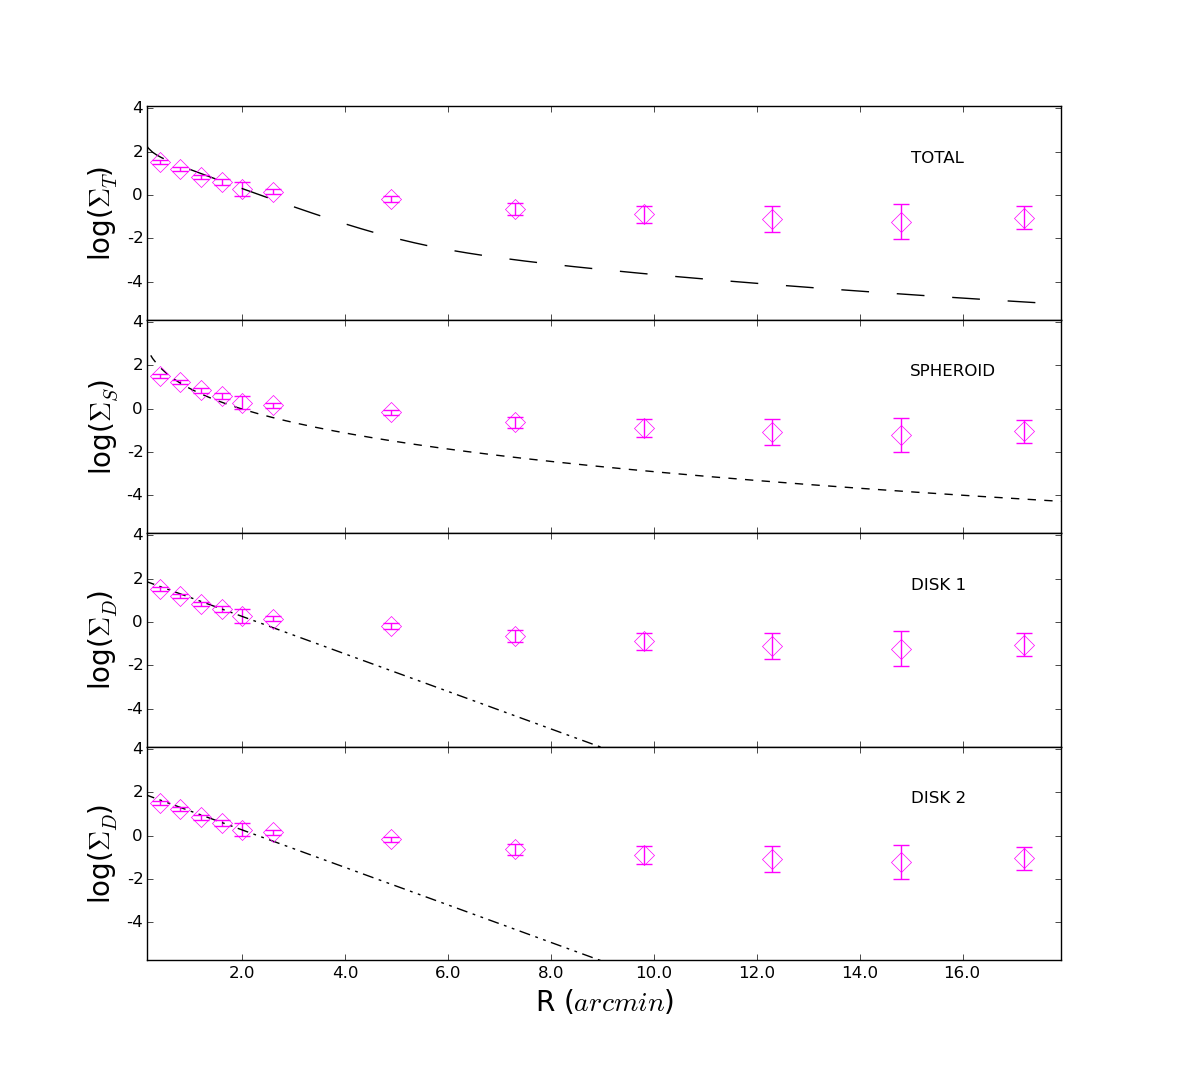
\includegraphics[scale=0.3]{5866dens3.png}
	\caption{GC number density, from \citet{hargis}, versus light profiles following GALFIT analysis. We found NGC 5866 to be well-fitted when considering two disk components. Nevertheless, there's a clear mismatch between GC number density and the light profiles after 5Kpc.}
\end{figure}

\begin{figure}[h]
	\centering
	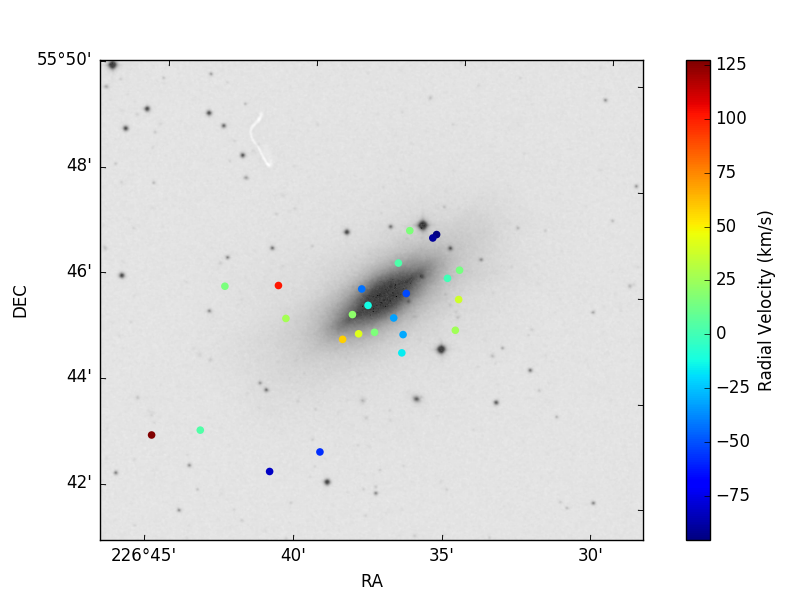
\includegraphics[scale=0.5]{5866vmap.png}
	\caption{Velocity map for spectroscopic GCs from SLUGGS, after smoothing using Adaptive Kernel Smoothing (AKS) \citep{cocatto}.}
\end{figure}

\bibliography{ref}

\end{document}
